\documentclass{beamer}

\usetheme[progressbar=foot,numbering=fraction]{metropolis}



\usepackage{appendixnumberbeamer}


%centrogeo orange
\definecolor{beamer@centrogeo}{RGB}{219,132,61}

%rareblue
\definecolor{beamer@centrogeo}{RGB}{2, 104, 161}

%itq orange
\definecolor{beamer@centrogeo}{RGB}{239, 158, 9}

% centrogeo brown
\definecolor{color2}  {RGB}{110,60,20}

\definecolor{color2}  {RGB}{61, 88, 122}

%centrogeo light orange
\definecolor{beamer@centrogeoLightOrange} {RGB}{255,172,101}% 

\definecolor{beamer@centrogeoLightOrange} {RGB}{61, 104, 161}% 

%https://www.centrogeo.org.mx/lgac-ciencias-de-informacion-geoespacial/lgac-cig-ciencias-de-informacion-geoespacial


\setbeamercolor{normal text}{fg=black,bg=white}
\setbeamercolor{alerted text}{fg=beamer@centrogeoLightOrange}
\setbeamercolor{example text}{fg=green!50!black}

\setbeamercolor{structure}{fg=color2}

\setbeamercolor{background canvas}{parent=normal text}
\setbeamercolor{background}{parent=background canvas}
	
\setbeamercolor{palette primary}{fg=white,bg=beamer@centrogeo} % changed this
\setbeamercolor{palette secondary}{use=structure,fg=structure.fg!100!green} % changed this
\setbeamercolor{palette tertiary}{use=structure,fg=structure.fg!100!green}



\usepackage[spanish, english]{babel}
\usepackage[utf8]{inputenc}

\usepackage{booktabs}
\usepackage[scale=2]{ccicons}
\usepackage{url}
%\usepackage{subfig}
\usepackage{subcaption}

\usepackage{caption}




%\usepackage{dsmath}

\usepackage{pgfplots}
\usepgfplotslibrary{dateplot}

\usepackage{xspace}
\newcommand{\themename}{\textbf{\textsc{metropolis}}\xspace}

\usepackage{algorithm}% http://ctan.org/pkg/algorithms
\usepackage[noend]{algpseudocode}

\usepackage{graphicx}
%\usepackage{subcaption}
\usepackage{bibentry}
\usepackage{verbatim}
\usepackage{fancyvrb}
\usepackage{moreverb}



\titlegraphic{
%\includegraphics[height=1.0cm]{figures/logo_cicige_L.png} \hfill  


\includegraphics[height=1.5cm]{TecNM_logo.png}  
\hfill 

\includegraphics[height=1.5cm]{itq.png} \hfill 
%5\includegraphics[height=0.9cm]{figures/EscudoDeLaUAQ.jpg}

}

\title{Internet de las Cosas:  Unidad 2}
\subtitle{Sensores y actuadores}


\author{Dr. Rodrigo López Farías. \\}

\institute{Instituto Tecnológico de Querétaro \\ Ingeniería en Sistemas Computacionales}

\date{Ciclo escolar Ene-Junio 2020}


\begin{document}

\frame{\maketitle}


\begin{frame}{Índice}
  \setbeamertemplate{section in toc}[sections numbered]
  \tableofcontents[hideallsubsections]
\end{frame}





\section{Programación de Entrada y Salida de Propósito General de la tarjeta de desarrollo}

\begin{frame}{Estructura Arduino}

\begin{figure}
\centering
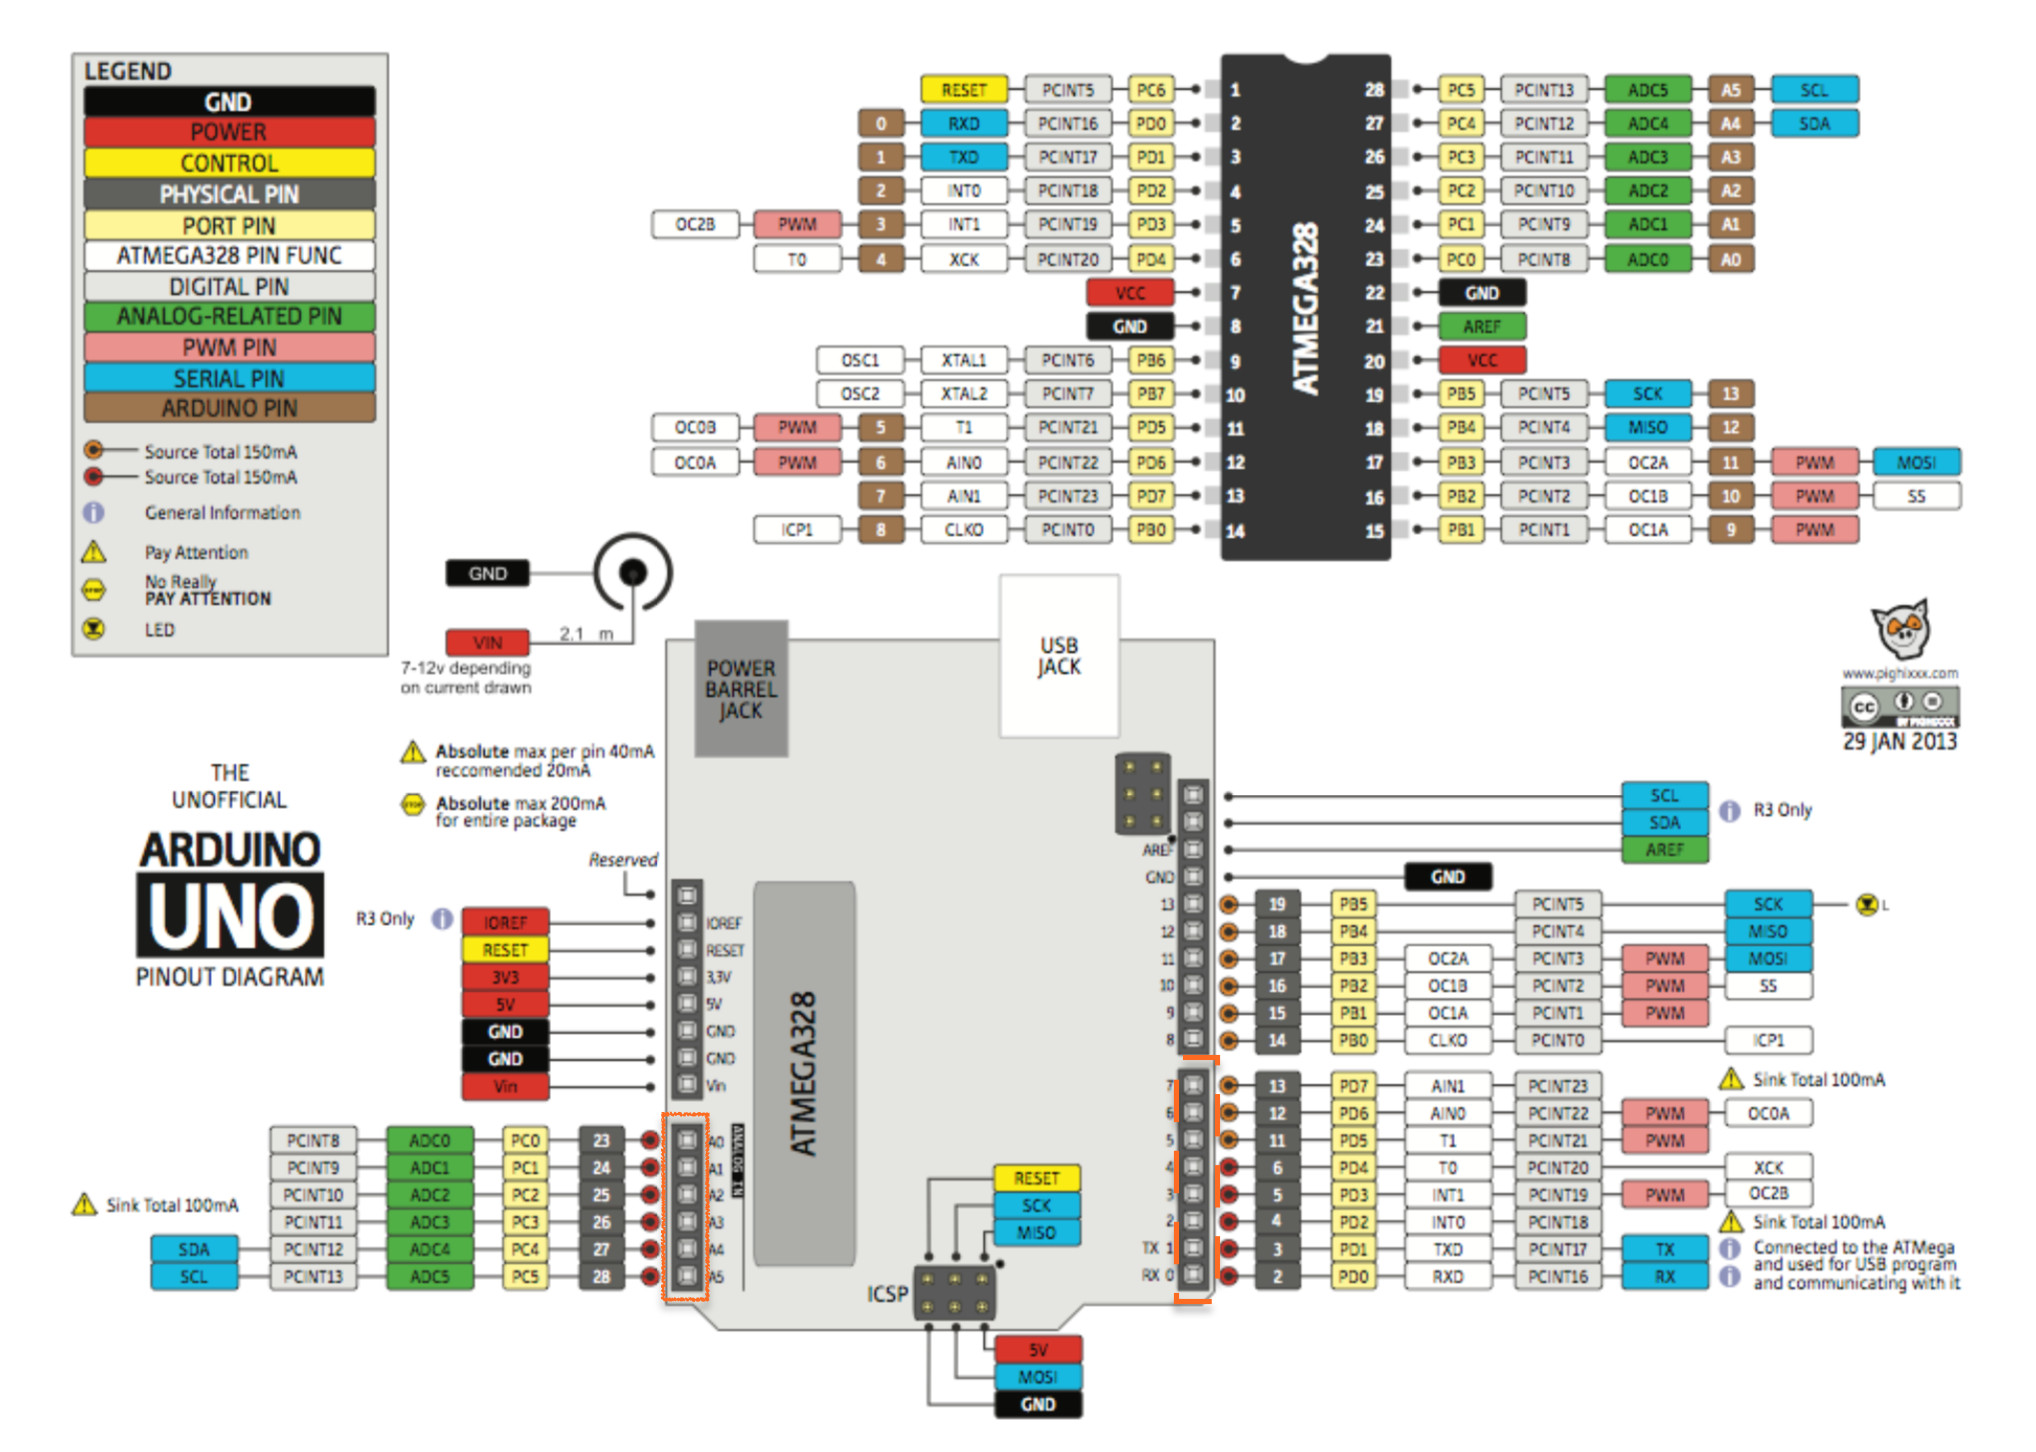
\includegraphics[width=0.7\textwidth]{figures/arduinounoref.png}
\caption{The Unofficial ARDUINO UNO Pinout Diagram \footnote{http://marcusjenkins.com/arduino-pinout-diagrams/} }
\end{figure}

\end{frame}


\section{Pines de entrada y salida}

\begin{frame}{Precauciones básicas}

\begin{itemize}
\item La tarjeta tiene 14 pines de entrada y salida digitales
\item Tiene 6 pines analógicos para lecturas análogas que tienen un rango definido.
\item Las entradas y salidas funcionan con un voltaje de 0V a 5V.
\item Máxima corriente por pin son 40mA.
\item Arduino se alimenta de tres maneras: por el USB (5V), pines de alimentación(5V) y por el Jack (alimentación entre 7V y 12V).
\item Se recomienda usar el USB solo para cargar programas. 
\item La fuente recomendada debe ser máximo 12 Volts corriente directa. La corriente puede variar ya que el Arduino solo consume la corriente necesaria.
%https://www.aladuino.com.mx/blog/limites-de-voltaje-corriente-y-alimentacion-del-arduino/
\end{itemize}

\end{frame}


\begin{frame}{Precauciones básicas para uso de los pines E\/S}

\begin{itemize}
\item Los pines soportan una corriente máxima de 40mA de entrada y salida a 5Volts.
\item Controlar la corriente requerida por los dispositivos conectados a la placa. 
\item Recordando Ley de Ohm
$$V = R \times I$$
\end{itemize}


\end{frame}


\begin{frame}{Precauciones básicas para uso de los pines E\/S}

Ejercicio:

Qué debo hacer si quiero conectar un componente (led) que utiliza a lo mas 20mA (0.02A) de corriente y la placa Arduino provee 5V? Respuest: utilizar una resistencia de al menos:

$$\frac{5V}{0.02A} <= R $$

Solución: despejando la resistencia.

Al determinar el valor de la resistencia, identificarla utilizando el código de colores \footnote{https://www.inventable.eu/paginas/ResCalculatorSp/ResCalculatorSp.html}

Se aconseja utilizar en este caso una resistencia mas grande para para no hacer trabajar la placa de Arduino al límite. e.g., emplear 5mA.


\end{frame}

\begin{frame}{Precauciones básicas para uso de los pines E\/S}

\begin{itemize}
\item Utilizar una fuente de voltaje externa (9V-12V) para poder proveer de niveles de corriente adecuados a los componentes conectados.
\item Aislar con carcasa para evitar el contacto con líquidos y estática.
\item Sensores que requieran de mas energía para funcionar, se requiere que se alimenten de manera independiente.
\item Utilizar multímetro para verificar voltaje y corriente.
\end{itemize}

\end{frame}



\begin{frame}{Características de lo Pines digitales de Arduino Uno}

\begin{itemize}
\item Entrada - Salida Digital: pulso alto 1 es sobrepasar el umbral de 3V y pulso bajo 0 a partir de 2V.
\item Pines digitales se definen como de entrada o salida con la función pinMode(\textit{pinNumber,INPUT xor OUTPUT}) ejemplo para definir una salida:
\begin{itemize}
\item pinMode(2,OUTPUT)
\end{itemize}
\item Ejemplo para escribir en un pin de salida utilizando la función pinWrite:
\begin{itemize}
\item pinWrite(3,[HIGH \ LOW])
\end{itemize}
Donde HIGH: 1 y LOW : 0
\end{itemize}

\end{frame}


\section{Desarrollo de programas para actuadores. (Básico)}

\begin{frame}{Ventana principal Arduino}


\begin{figure}
\centering
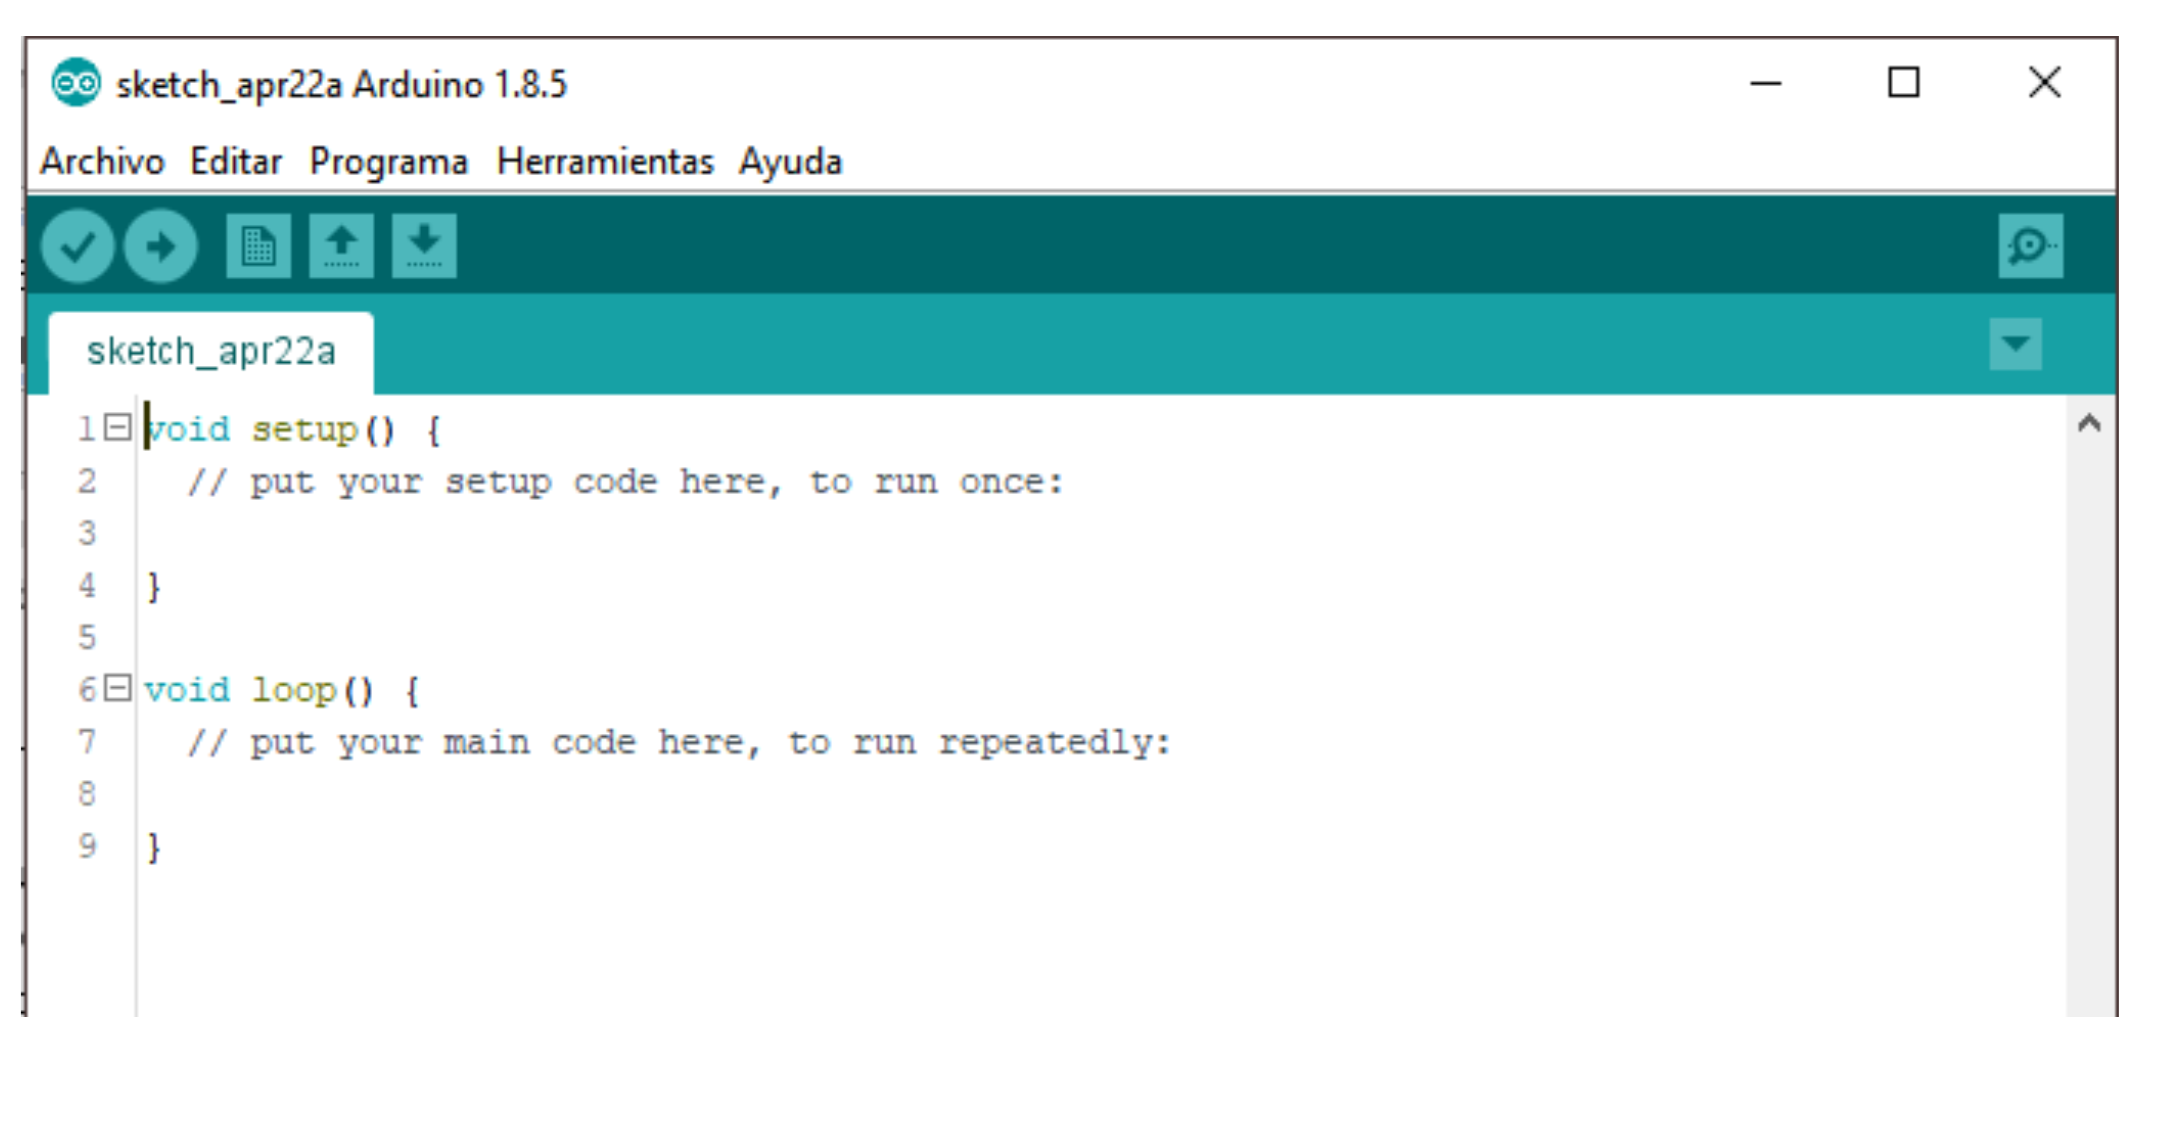
\includegraphics[width=0.9\textwidth]{figures/arduinoide.png}
\caption{Ventana principal del IDE de Arduino}
\end{figure}

\end{frame}


\begin{frame}[fragile]
{Código Ejemplo, programación pin de salida}
\tiny
\begin{verbatim}[tabsize=4]


#define LED 2 //Damos el alias a nuestro pin 2.
void setup(){
	pinMode(LED,OUTPUT); //Definimos el pin LED como salida. 
}

void loop(){ //Definimos nuestra secuencia.
	digitalWrite(LED,HIGH); //Mandamos un ALTO al LED.
	delay(1000); //Tiempo en que permanece el LED prendido “un segundo”. 		digitalWrite(LED,LOW); //Mandamos un BAJO al LED.
	delay(1000); //Tiempo en que permanece el LED apagado “un segundo”. 
}

\end{verbatim}
\end{frame}

\section{Desarrollo de programas para sensores y actuadores (Básico)}

\begin{frame}


\begin{figure}
\centering
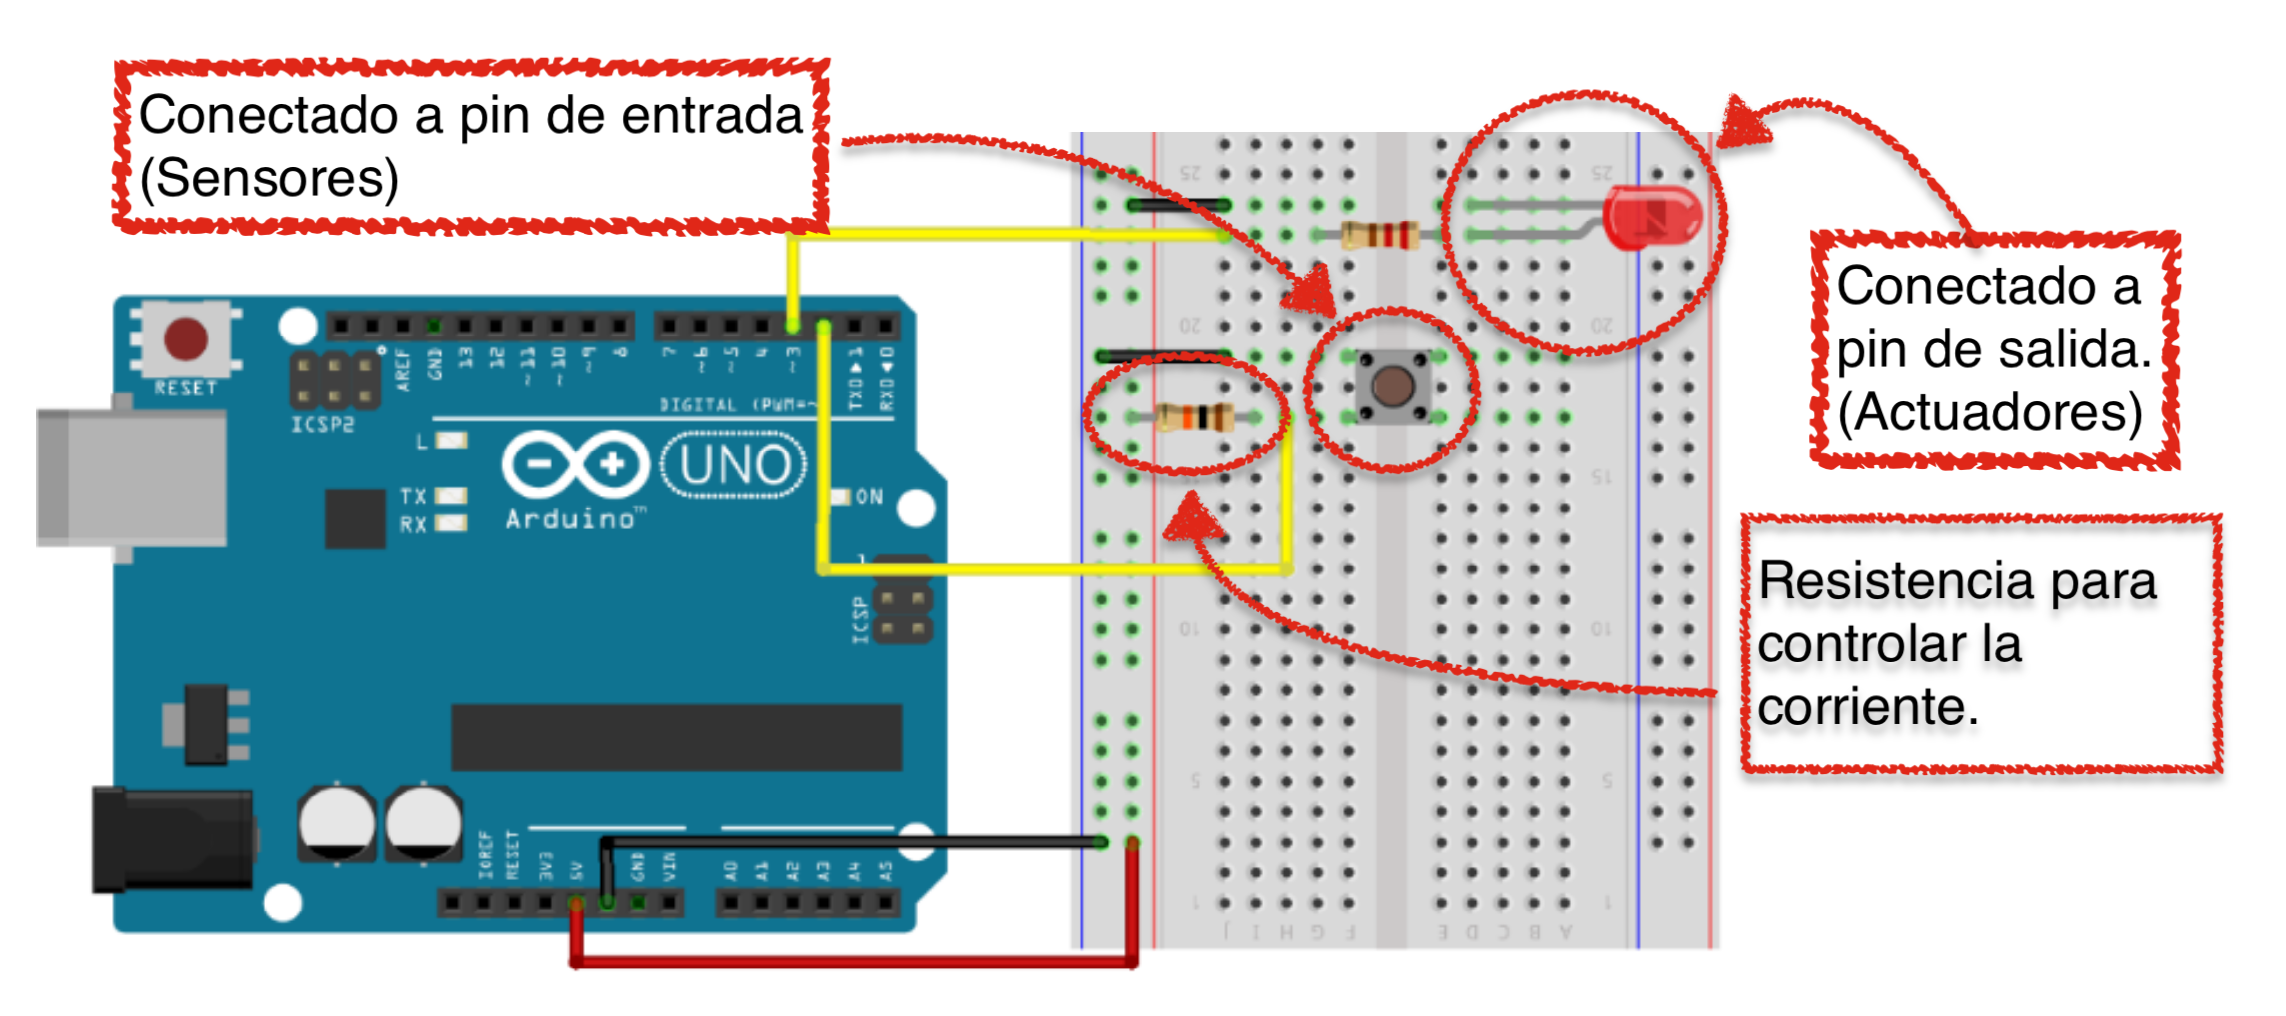
\includegraphics[width=0.9\textwidth]{figures/esquemaiodigital.png}
\caption{Esquema Digital Básico pines de salida}
\end{figure}



\end{frame}

\begin{frame}[fragile]
{Código Ejemplo, programación pin de entrada y salida}


\tiny

\begin{verbatimtab}

#define LED 2  //Damos el alias a nuestro pin 2.
#define Push 3 //Damos el alias a nuestro pin 3.
byte Push_lee = 0;
void setup(){
	pinMode(LED,OUTPUT); //Definimos el pin LED como salida. 
	pinMode(Push,INPUT); //Definimos el pin Push como entrada. 
}

//Definimos el algoritmo principal
void loop(){
		Push_lee = digitalRead(Push); //Almacenamos en la variable la lectura del 	pulsador.
	if(Push_lee == 1){ 			//Cond. que si tenemos el valor de 1 entra en el.
		digitalWrite(LED,HIGH); 
	}else{
		digitalWrite(LED,LOW); //Mandamos un BAJO al LED.
	}
}

\end{verbatimtab}

\end{frame}


\section{Desarrollo de programas para sensores y actuadores analógicos (Básico) y Desarrollo de programas para adquisici\'on de datos}


\begin{frame}{Sensores Analógicos}

La señal analógica tiene Valores continuos en un rango entre 0V y 5V.

Esta señal se convierte  a señal digital por medio de un transductor.

Arduino UNO tiene 6 puertos analógicos del A0 al A5

Estos puertos son de entrada analógica o entrada y salida digital.

El firmware (bootloader) de Arduino tiene una resolución por defecto de 10 bits $2^{10}=1024$ valores. (de 0 a 255)

Se puede cambiar el voltaje máximo de referencia con el pin AREF.

\end{frame}

\subsection{Sensor análogo: conversión analógico digital}

\begin{frame}
Para poder trabajar con los valores entrada de la señal analógica con el microcontrolador, es necesario convertirla primero una señal digital por medio de esta fórmula de escalamiento.



$$V_{dig} =  \frac{ V (2^n - 1) }{V_{ref}} $$

Donde: $V$ es el voltaje analógico de entrada. $2^n-1$ es el valor entero positivo máximo del convertidor y $V_{ref}$ es el valor de voltaje (máximo) de referencia. Esta operación Arduino la hace internamente. 

Pregunta: Cómo utilizar la fórmula para aplicar un nivel de voltaje desde la tarjeta Arduino uno a un pin de salida? 

\end{frame}


\begin{frame}[fragile]
Código de ejemplo lectura de un Potenciómetro desde un pin analógico.

\tiny
\begin{verbatimtab}
#define POT A0
int LeePot;
void setup() {
	\\ velocidad de transmisión en baudios (bits/seg)
  Serial.begin(9600); 
  pinMode(POT,INPUT);
}
void loop() {
  LeePot = analogRead(POT);
  Serial.println(LeePot);
  delay(50);
}
\end{verbatimtab}

Página 49.
\end{frame}


\begin{frame}{Actuadores analógicos.}
Arduino funciona con un microcontrolador que es de naturaleza digital. 
Lo que se hace es representar esa señal analógica con información digital usando una técnica llamada Modulación por Ancho de Pulso (\textit{Pulse Width Modulation PWM}) la cual:

\begin{itemize}
\item Una señal analógica se representa con una señal cuadrada que adquiere solo valores Alto o Bajo.
\item El porcentaje de la duración de el valor en alto da lugar al ancho de pulso (ciclo de trabajo\footnote{Es la fraccion de un periodo el cual la senal esta activa}) que representa un valor en la señal analógica.
\item Tiene resolución de 8 bits ($2^8$)
\end{itemize}
Arduino Uno cuenta con 6 pines en total que pueden trabajar con PWM. \footnote{Ver pag 55 del curso Arduino Básico de Saenz Flores.}

\end{frame}

\begin{frame}[fragile]Ejemplo: Programa escritura analógica en un pin.

Para escribir con estos pines usamos la funci\'{o}n analogWrite([pin/alias],[valor/variable]);

\tiny
\begin{verbatimtab}

#define LED 3
void setup() {
	#Definimos el pin LED como salida 
 	pinMode(LED,OUTPUT); 
}

#Programa principal dentro del loop
void loop() {
	
  for(int i = 1; i <= 255; i++){
    analogWrite(LED,i);
    delay(10);
    }
    delay(1000);
  for(int i = 255; i >= 1; i--){
    analogWrite(LED,i);
    delay(10);
    }
  delay(1000);
}
\end{verbatimtab}

Si esta conectado un led al pin LED a la placa de Arduino. Que es lo que hace este programa.



\end{frame}


\begin{frame}{Tarea: Práctica 2}

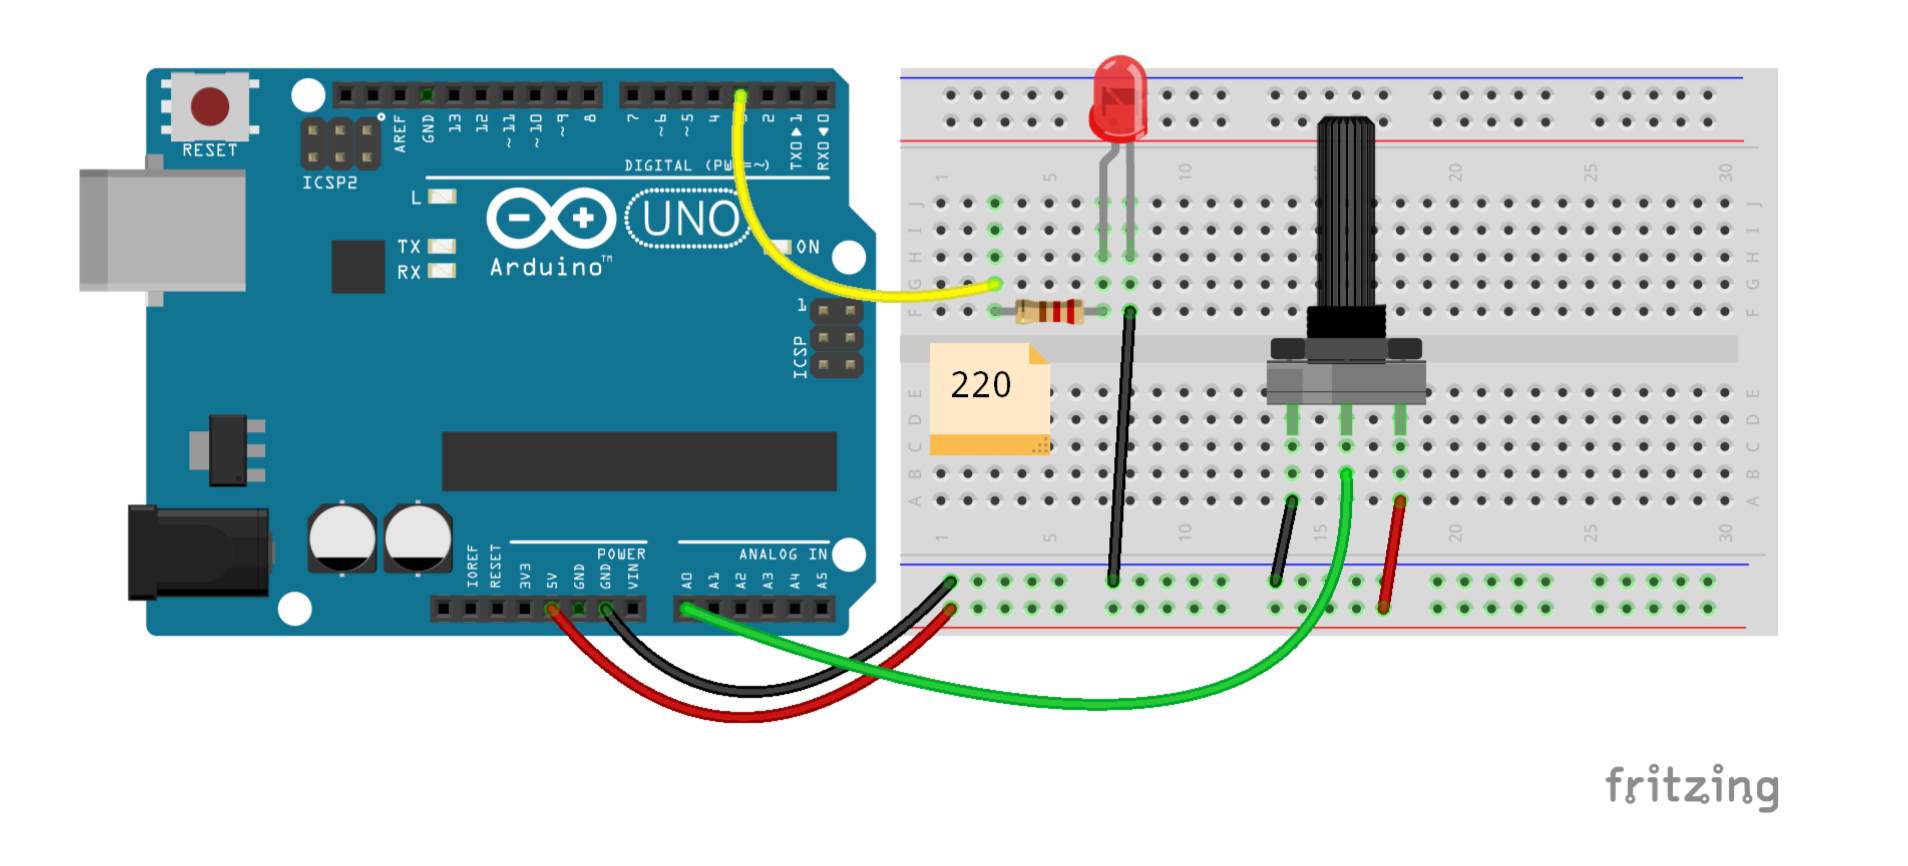
\includegraphics[width=0.9\textwidth]{figures/tarea2.png}

\end{frame}




\subsection{Leer datos desde diferentes tipos de Sensores.  (IR*, micrófonos, cámaras, GPS*, acelerómetros*, giroscopios*, sensores ultrasónicos*, etc...)}

\section{Desarrollo de programas para actuadores}
%: Motores a pasos, pantallas LCD, bocinas, etc.

\begin{frame}

\end{frame}

\section{Estimación de frecuencias de muestreo y ancho de bits para diferentes sensores}

\begin{frame}

\end{frame}










\end{document}